\begin{frame}[fragile]

  {\Huge Sparse Solvers}

  \vspace{10pt}

  {\large Gauss-Seidel Preconditioners}

  \vspace{20pt}

  \textbf{Learning objectives:}
  \begin{itemize}
    \item {Multicolor Gauss-Seidel}
    \item {Cluster Gauss-Seidel}
    \item {Two-Stage Gauss-Seidel}
  \end{itemize}

  \vspace{-20pt}

\end{frame}

%==========================================================================

\begin{frame}[fragile]{Multicolor Gauss-Seidel}
\textbf{Multicolor Gauss-Seidel}

Gauss-Seidel (GS) method for solving $A\mathbf{x} = \mathbf{b}$ updates one entry of the unknown at a time:

For $i = 1..M$:
\[ \mathbf{x}_i := (\mathbf{b}_i - \sum_{j=1}^{N} A_{ij}\mathbf{x}_j) / A_{ii}\]

\begin{itemize}
  \item Standard GS is sequential: updates to $\mathbf{x}_i$ are affected by previous updates to $\mathbf{x}_j$ in the same iteration (where $j < i$)
  \item Treating A as a graph's adjacency matrix, $A_{ij} \neq 0$ if vertices $i$ and $j$ are adjacent
  \item Suppose a coloring is computed for this graph, and $\mathit{Color}(i) = \mathit{Color}(j)$.
  \item then $\mathbf{x}_j$ does not directly affect the updated value of $\mathbf{x}_i$
\end{itemize}
\end{frame}

\begin{frame}[fragile]{Multicolor Gauss-Seidel}
\textbf{Using KokkosKernels Multicolor GS}

KokkosKernels supports preconditioning with multicolor GS. Rows with the same color are updated in parallel.

\begin{code}
  #include "KokkosSparse_gauss_seidel.hpp"
  // Handle creation
  KokkosKernels::KokkosKernelsHandle<...> handle;
  handle.create_gs_handle(KokkosSparse::GS_POINT);
  // Symbolic setup
  KokkosSparse::Experimental::gauss_seidel_symbolic(
    &handle, numRows, numCols,
    A.graph.row_map, A.graph.entries, graphIsSymmetric);
  // Numeric setup
  KokkosSparse::Experimental::gauss_seidel_numeric(
    &handle, numRows, numCols,
    A.graph.row_map, A.graph.entries, A.values,
    graphIsSymmetric);
\end{code}
\end{frame}

\begin{frame}[fragile]{Multicolor Gauss-Seidel}
\textbf{Using KokkosKernels Multicolor GS, continued}

KokkosKernels supports parallel preconditioning with multicolor GS.

\begin{code}
  KokkosSparse::Experimental::forward_sweep_gauss_seidel_apply(
    &handle, numRows, numCols,
    A.graph.row_map, A.graph.entries, A.values,
    x, b, initZeroX, updateCachedB, omega, numSweeps);
  // --- or ---
  KokkosSparse::Experimental::backward_sweep_gauss_seidel_apply(
    &handle, numRows, numCols,
    A.graph.row_map, A.graph.entries, A.values,
    x, b, initZeroX, updateCachedB, omega, numSweeps);
  // --- or ---
  KokkosSparse::Experimental::symmetric_gauss_seidel_apply(
    &handle, numRows, numCols,
    A.graph.row_map, A.graph.entries, A.values,
    x, b, initZeroX, updateCachedB, omega, numSweeps);
  // Clean up
  handle.destroy_gs_handle();
\end{code}
\end{frame}

\begin{frame}[fragile]{Multicolor Gauss-Seidel}
\textbf{Using KokkosKernels Multicolor GS}

\begin{itemize}
  \item Algorithm called \verb!POINT! because individual rows of the matrix are colored, as opposed to blocks/clusters
  \item \verb!graphIsSymmetric!: whether the matrix is structurally symmetric.
    If false, must symmetrize before coloring.
  \item \verb!initZeroX!: whether to zero out $\mathbf{x}$ before starting
  \item \verb!updateCachedB!: whether on the first apply, or $\mathbf{b}$ has changed since the last apply
  \item \verb!omega!: damping factor for successive over-relaxation (default is 1.0)
  \item \verb!numSweeps!: how many applications to perform. For symmetric apply, forward+back counts as 1 application.
\end{itemize}

\end{frame}

\begin{frame}[fragile]{Cluster Gauss-Seidel}
\textbf{Cluster GS}

\begin{itemize}
  \item In Multicolor GS, an independent row $j$ does not \emph{directly} affect the updated value of $\mathbf{x}_i$, but it can affect it \emph{indirectly}.
  \item For example, if $i$ and $j$ have the same color and are separated by $k$,
    then information is not transferred from $\mathbf{x}_i$ to $\mathbf{x}_j$ through $\mathbf{x}_k$ within a sweep.
  \item This is why multicolor GS usually gives a slightly worse answer than sequential GS.
  \item To help with this, cluster GS coarsens the graph and applies GS sequentially within a cluster.
\end{itemize}
\end{frame}

\begin{frame}[fragile]{Cluster Gauss-Seidel}
\textbf{Cluster GS}
Example:
\begin{code}
  handle.create_gs_handle(
    KokkosSparse::CLUSTER_BALLOON, clusterSize);
\end{code}
\begin{itemize}
  \item ``Balloon'' is the coarsening algorithm (others may be added in the future)
  \item \verb!clusterSize! is the coarsening factor (an integer larger than 1, but should be small compared to the number of rows)
  \item The symbolic, numeric and apply interface is the same as multicolor (\verb!POINT!)
\end{itemize}
\end{frame}

\begin{frame}[fragile]{Two-Stage Gauss-Seidel}
\textbf{Two-Stage GS}
\begin{itemize}
  \item Hybrid of the Jacobi and Gauss-Seidel methods
  \item Formulates Gauss-Seidel as a lower or upper triangular solve (for forward and backward sweeps, respectively),
    and uses some number of Jacobi sweeps as an approximation for this solve.
\end{itemize}

Usage:

\begin{code}
  handle.create_gs_handle(KokkosSparse::TWO_STAGE);
\end{code}
\end{frame}

\begin{frame}[fragile]{Exercise}
\textbf{GS: Exercise}
\begin{itemize}
  \item \verb!Intro-Full/Exercises/kokkoskernels/GaussSeidel!
  \item Generates a small, diagonally dominant system
  \item Fill in the neccesary calls to set up and use one of the GS algorithms as an iterative solver
\end{itemize}
\end{frame}

\begin{frame}[fragile]{Summary}
\textbf{Summary: Gauss-Seidel}
\begin{itemize}
  \item Multicolor Gauss-Seidel
  \begin{itemize}
    \item Uses coloring to find independent rows
  \end{itemize}
  \item Cluster Gauss-Seidel
  \begin{itemize}
    \item Like multicolor but coarsens graph first
  \end{itemize}
  \item Two-Stage Gauss-Seidel
  \begin{itemize}
    \item Hybrid Gauss-Seidel/Jacobi-Richardson
  \end{itemize}
\end{itemize}

The best choice depends on the problem.

\end{frame}

%==========================================================================

\begin{frame}[fragile]

  {\Huge Sparse Solvers 2}

  \vspace{10pt}

  {\large Sparse factorization and triangular solver.}

  \vspace{20pt}

  \textbf{Learning objectives:}
  \begin{itemize}
    \item {Sparse incomplete LU factorization}
    \item {Sparse triangular solvers}
  \end{itemize}

  \vspace{-20pt}

\end{frame}

%==========================================================================

\begin{frame}[fragile]{Overview}
\textbf{SPARSE SPILUK and SPTRSV}

KokkosKernels supports preconditioning with sparse incomplete LU factorization coupled with sparse triangular solvers.

%\[ A\mathbf{x} = b \Leftrightarrow M^{-1}A\mathbf{x} = M^{-1}\mathbf{b} \]

\begin{itemize}
%  \item Use case: ILU to generate LU factorization for preconditioner used with linear iterative solvers, robust for elliptic PDE's, does not work well for indefinite systems
  \item \textbf{SPILUK}: Sparse k-level incomplete LU factorization
  \begin{itemize}
    \item Computes sparse lower triangular matrix $L$ and upper triangular matrix $U$ such that $M = LU$ is "similar" to $A$
    \item $k = 0$: No additional fill-in. $G(L+U) = G(A)$
    \item $k > 0$: Increased fill level improves accuracy
  \end{itemize}
  \vspace{1em}
  \item \textbf{SPTRSV}: Sparse triangular solver
  \begin{itemize}
    \item Apply ILU: $\mathbf{z} = M^{-1}\mathbf{r} \Leftrightarrow z = (LU)^{-1}\mathbf{r} \Leftrightarrow z = U^{-1}(L^{-1}\mathbf{r})$
    \item L,U reused by triangular solver to apply preconditioning during linear solver iterations
  \end{itemize}
\end{itemize}

\end{frame}

\begin{frame}[fragile]{SPILUK}
\textbf{SPILUK usage}

  \begin{itemize}
    \item ILU(k): requires matrices in "Crs" format
    \item Symbolic phase on host (serial):
    \begin{itemize}
      \item Construct nonzero patterns of L and U
      \item Perform level-scheduling to group independent rows into levels based on L's sparsity pattern. Level-scheduling results stored within a handle for reuse
    \end{itemize}
    \item Numeric phase (parallel) fill data to the nonzero patterns based on level-scheduling results found in the symbolic phase
    \item Algorithm options:
    \begin{itemize}
      \item SEQLVLSCHD\_RP: using range policy parallelism for numeric phase
      \item SEQLVLSCHD\_TP1: using team policy parallelism for numeric phase
    \end{itemize}
  \end{itemize}

\end{frame}

\begin{frame}[fragile]{SPILUK}
\textbf{SPILUK: Interface}

  \begin{itemize}
    \item \{A,L,U\}\_rowmap: Arrays storing row pointer offset, as a 1-D Kokkos::View
    \item \{A,L,U\}\_entries: Arrays storing column indices, as a 1-D Kokkos::View
    \item \{A,L,U\}\_values: Arrays storing corresponding matrix values, as a 1-D Kokkos::View
    \item Handle: Stores internal data structures from symbolic phase
    \begin{itemize}
      \item Input: SPILUKAlgorithm, number of rows, est. number of nonzeros L, est. number of nonzeros of U
      \item Templated on rowmap data type (size\_type), entries ordinal type (lno\_t), values scalar type (scalar\_t), execution space, "persistent" memory space, "temporary" memory space (unused here)
    \end{itemize}
  \end{itemize}

\end{frame}

\begin{frame}[fragile]{SPILUK}
\textbf{SPILUK: Interface}

\begin{itemize}
  \item<2-> Include header file
    \begin{code}[keywords={parallel_reduce,for,int,double}, basicstyle=\tiny, breaklines=true]
#include "KokkosSparse_spiluk.hpp"
  //SPILUK in Experimental namespace - interface may evolve
using namespace KokkosKernels::Experimental;
    \end{code}

  \item<3-> Create opaque handle
    \begin{code}[keywords={parallel_reduce,for,int,double}, basicstyle=\tiny, breaklines=true]
KokkosKernelsHandle 
<size_type, lno_t, scalar_t, exec_space, mem_space, mem_space> kh;
    \end{code}

  \item<4-> Create the spiluk handle - requires estimate for nnz of L, U
    \begin{code}[keywords={parallel_reduce,for,int,double}, basicstyle=\tiny, breaklines=true]
nnzL = nnzU = EXPAND_FACT*A.nnz()*(fill_lev+1); // EXPAND_FACT set by user
kh.create_spiluk_handle(SPILUKAlgorithm, nrows, nnzL, nnzU);
    \end{code}

  \item<5-> Call symbolic routine
    \begin{code}[keywords={parallel_reduce,for,int,double}, basicstyle=\tiny, breaklines=true]
spiluk_symbolic(&kh, fill_level, A_rowmap, A_entries, 
                    L_rowmap, L_entries, U_rowmap, U_entries);
    \end{code}

  \item<6-> Call numeric routine
    \begin{code}[keywords={parallel_reduce,for,int,double}, basicstyle=\tiny, breaklines=true]
spiluk_numeric(&kh, fill_level, A_rowmap, A_entries, A_values, 
                                L_rowmap, L_entries, L_values, 
                                U_rowmap, U_entries, U_values);
    \end{code}

\end{itemize}

\end{frame}


\begin{frame}[fragile]{SPTRSV}
\textbf{SPTRSV usage}

  \begin{itemize}
    \item Sparse triangular solver: $\{L,U\}\mathbf{x} = \mathbf{b}$
    \begin{itemize}
      \item Fallback solver options
      \item Supernode-based solver options
    \end{itemize}
    \item Fallback implementation and TPL options:
    \begin{itemize}
      \item Symbolic phase analyzes matrix structure
      \begin{itemize}
        \item Level-scheduling employed to expose parallelism to solver
        \item All rows within a level can be solved independently in parallel
        \item Symbolic phase results stored within handle for reuse
      \end{itemize}
      \item Solve phase: Uses level-set information from symbolic to execute in parallel
      \item Separate phases allows reuse of symbolic phase / level scheduling information
      \begin{itemize}
        \item Use case: As direct solver for preconditioner for iterative solver methods, following factorization
      \end{itemize}
    \end{itemize}
  \end{itemize}

\end{frame}


\begin{frame}[fragile]{SPTRSV}
\textbf{SPTRSV usage}

  \begin{itemize}
      \item Algorithm options:
      \begin{itemize}
        \item SEQLVLSCHD\_TP1: Seq. level scheduling, solver hierarchical parallelism
        \item SEQLVLSCHD\_TP1CHAIN: Seq. level scheduling, solver hierarchical parallelism
        \begin{itemize}
          \item "Chaining" of consecutive levels with few rows into single kernel launch
          \item Reduces number of kernel launches for levels bound by launch overhead, e.g. banded matrices
        \end{itemize}
        \item SPTRSV\_CUSPARSE: Wrapper of NVIDIA's CuSPARSE triangular solver
      \end{itemize}
  \end{itemize}

\end{frame}


\begin{frame}[fragile]{SPTRSV}
\textbf{SPTRSV: Interface}
  \begin{itemize}
    \item \{L,U\}\_rowmap: Arrays storing row pointer offset, as a 1-D Kokkos::View
    \item \{L,U\}\_entries: Arrays storing column indices, as a 1-D Kokkos::View
    \item \{L,U\}\_values: Arrays storing corresponding matrix values, as a 1-D Kokkos::View
    \item Handle: Stores internal data structures from symbolic phase
    \begin{itemize}
      \item Input: SPTRSVAlgorithm, number of rows, boolean (is lower triangular)
      \item Templated on rowmap data type (size\_type), entries ordinal type (lno\_t), values scalar type (scalar\_t), execution space, "persistent" memory space, "temporary" memory space (unused here)
    \end{itemize}
    \item \{x,b\}: Dense vectors as rank-1 Views
  \end{itemize}

\end{frame}


\begin{frame}[fragile]{SPTRSV}
\textbf{SPTRSV: Interface}

\begin{itemize}
  \item<2-> Include header file
  \begin{code}[keywords={parallel_reduce,for,int,double}, basicstyle=\tiny, breaklines=true]
#include "KokkosSparse_sptrsv.hpp"
//SPTRSV in Experimental namespace - interface may evolve
using namespace KokkosKernels::Experimental;
  \end{code}

  \item<3-> Create opaque handle
  \begin{code}[keywords={parallel_reduce,for,int,double}, basicstyle=\tiny, breaklines=true]
KokkosKernelsHandle 
<size_t, lno_t, scalar_t, exec_sp, mem_sp, mem_sp> kh;
  \end{code}

  \item<4-> Create sptrsv handle - separate handles required for L and U
  \begin{code}[keywords={parallel_reduce,for,int,double}, basicstyle=\tiny, breaklines=true]
kh.create_sptrsv_handle(SPTRSVAlgorithm, nrows, lower_tri);
  \end{code}

  \item<5-> Call symbolic analysis
  \begin{code}[keywords={parallel_reduce,for,int,double}, basicstyle=\tiny, breaklines=true]
sptrsv_symbolic(&kh, rowmap, entries, values);
  \end{code}

  \item<6-> Call solve
  \begin{code}[keywords={parallel_reduce,for,int,double}, basicstyle=\tiny, breaklines=true]
sptrsv_solve((&kh, rowmap, entries, values, b, x);
  \end{code}
\end{itemize}
\end{frame}

%%%%%

\begin{frame}[fragile]{SPTRSV supernode-based}
\textbf{SPTRSV supernode-based usage}

  \begin{itemize}
      \item Users responsible for reordering and factorization to provide supernode block info
      \item Metis and SUPERLU software was used for this during development of the algorithm
      \item Symbolic phase analyzes matrix structure
      \begin{itemize}
        \item Level-set scheduling of supernode blocks
        \item Internal data structures are setup to store blocks
        \item Symbolic phase results stored within handle for reuse
        \item Optional: Merge supernodes with matching sparsity pattern
      \end{itemize}
      \item Compute phase
      \begin{itemize}
        \item Copy triangular matrix data to internal data structures
        \item Optional: Invert diagonal blocks; apply inverse to off-diagonal blocks
      \end{itemize}
      \item Solve phase: Uses level-set information to execute in parallel
      \item Separate phases allows reuse of symbolic and compute
  \end{itemize}

\end{frame}


\begin{frame}[fragile]{SPTRSV supernode-based}
\textbf{SPTRSV supernode-based usage}

  \begin{itemize}
%    \item Use cases:
%      \begin{itemize}
%        \item Domain-decomposition based linear solvers relying on direct solver for local solution
%        \item Multi-grid preconditioners with local sptrsv for coarse grid solve
%      \end{itemize}
    \item Algorithm options:
    \begin{itemize}
      \item SUPERNODAL\_DAG: Applies batched TRSV/GEMV kernels to supernodes at each level, internally computes DAG for scheduling
      \item SUPERNODAL\_SPMV\_DAG: Applies SPMV at each level and requires inverted diagonal blocks, internally computes DAG for scheduling
      \item SUPERNODAL\_ETREE: Like SUPERNODAL\_DAG, scheduling based on user-provided etree (e.g. from SuperLU)
      \item SUPERNODAL\_SPMV: Like SUPERNODAL\_SMPV\_DAG, scheduling based on user-provided etree
    \end{itemize}
    \item For more details see: \scriptsize{I. Yamazaki, S. Rajamanicakm, N. Ellingwood “Performance Portable Supernode-based Sparse Triangular Solver for Manycore Architectures”, \url{https://dl.acm.org/doi/fullHtml/10.1145/3404397.3404428}}
  \end{itemize}

\end{frame}

\begin{frame}[fragile]{SPTRSV supernode-based}
\textbf{SPTRSV: Interface supernode-based}

  \begin{itemize}
    \item \{L,U\}.graph: StaticCrsGraph data structure containing rowmap offsets and column indices
    \item nsuper: Number of supernode blocks
    \item supercols: Array of supernode block sizes
    \item etree: (Optional) Used for level scheduling
    \item Handle: Stores internal data structures and matrix blocks from symbolic and compute
    \begin{itemize}
      \item Input: SPTRSVAlgorithm, number of rows, boolean (is lower triangular)
      \item Templated on rowmap data type (size\_type), entries ordinal type (lno\_t), values scalar type (scalar\_t), execution space, "persistent" memory space, "temporary" memory space (unused here)
    \end{itemize}
    \item \{x,b\}: Dense vectors as rank-1 Views
  \end{itemize}
\end{frame}

\begin{frame}[fragile]{SPTRSV supernode-based}
\textbf{SPTRSV: Interface supernode-based}

\begin{itemize}
  \item<2-> Include header file
  \vspace{-0.5em}
  \begin{code}[keywords={parallel_reduce,for,int,double}, basicstyle=\tiny, breaklines=true]
#include "KokkosSparse_sptrsv_supernode.hpp"
//SPTRSV in Experimental namespace - interface may evolve
using namespace KokkosKernels::Experimental;
  \end{code}

  \item<3-> Create opaque handle
  \vspace{-0.5em}
  \begin{code}[keywords={parallel_reduce,for,int,double}, basicstyle=\tiny, breaklines=true]
KokkosKernelsHandle 
<size_t, lno_t, scalar_t, exec_sp, mem_sp, mem_sp> kh;
  \end{code}

  \item<4-> Create sptrsv handle - separate handles for L and U
  \vspace{-0.5em}
  \begin{code}[keywords={parallel_reduce,for,int,double}, basicstyle=\tiny, breaklines=true]
khL.create_sptrsv_handle(SPTRSVAlgorithm::SUPERNODAL_SPMV_DAG, nrows, lower_tri);
khU.create_sptrsv_handle(SPTRSVAlgorithm::SUPERNODAL_SPMV_DAG, nrows, lower_tri);
  \end{code}

  \item<5-> Set options
  \vspace{-0.5em}
  \begin{code}[keywords={parallel_reduce,for,int,double}, basicstyle=\tiny, breaklines=true]
// whether to merge supernodes (false defaults)
khL.set_sptrsv_merge_supernodes (merge);

// invert diagonal blocks
khL.set_sptrsv_invert_diagonal (invert_diag);

// whether to apply diagonal-inversion to off-diagonal blocks
khL.set_sptrsv_invert_offdiagonal (invert_offdiag);
  \end{code}
\end{itemize}
\end{frame}

\begin{frame}[fragile]{SPTRSV supernode-based cont.}
\textbf{SPTRSV: Interface supernode-based}

\begin{itemize}

  \item<1-> Call symbolic analysis
  \begin{code}[keywords={parallel_reduce,for,int,double}, basicstyle=\tiny, breaklines=true]
sptrsv_supernodal_symbolic (nsuper, supercols.data (), etree, L.graph, &khL, L.graph, &khU);
  \end{code}

  \item<2-> Call compute
  \begin{code}[keywords={parallel_reduce,for,int,double}, basicstyle=\tiny, breaklines=true]
sptrsv_compute (&khL, L);
  \end{code}

  \item<3-> Call solve
  \begin{code}[keywords={parallel_reduce,for,int,double}, basicstyle=\tiny, breaklines=true]
sptrsv_solve (&khL, x, b);
  \end{code}
\end{itemize}
\end{frame}

%%

\begin{frame}[fragile]{Exercise}
\textbf{Use Case: Preconditioned Conjugate Gradient Solver}

Assume A and M are both symmetric and positive-definite

  \begin{columns}[t,onlytextwidth]
    \column{.45\textwidth}
      \vspace{-2em}
      \begin{center}
      \textbf{\tiny{Conjugate Gradient}}
      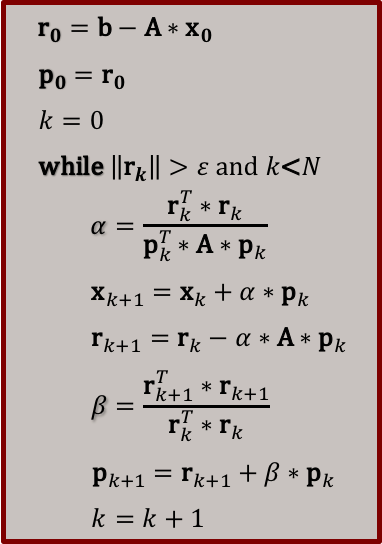
\includegraphics[scale=0.50]{figures/SPARSE-CGAlg}
      \vspace{-2em}
      \end{center}
    \column{.10\textwidth}
    \column{.45\textwidth}
      \vspace{-2em}
      \begin{center}
      \textbf{\tiny{Preconditioned Conjugate Gradient}}
      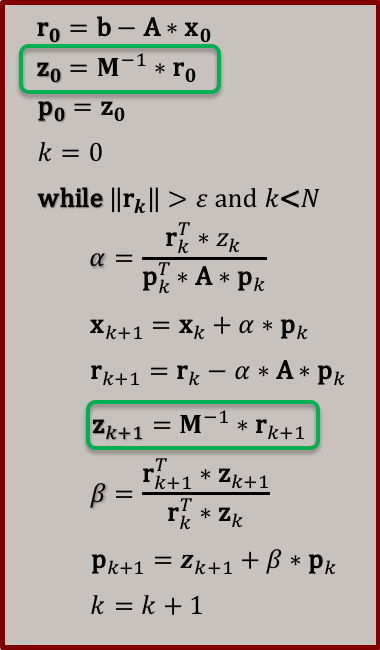
\includegraphics[scale=0.50]{figures/SPARSE-PrecondCGAlg}
      \vspace{-2em}
      \end{center}
  \end{columns}
\end{frame}

\begin{frame}[fragile]{Exercise}
\textbf{Use Case: Preconditioned Conjugate Gradient Solver}

Goal: Introduce preconditioning to a CG solver code

  \begin{columns}[t,onlytextwidth]
    \column{.55\textwidth}
      \vspace{1em}
      \\
      \begin{itemize}
      \item SPILUK: Yields factored M
      \item $M = LU \approx A$
      \item $M^{-1} = U^{-1}L^{-1}$
      \vspace{2em}
      \item SPTRSV: Apply twice for z
      \item $tmp = L \setminus r$ (Matlab notation)
    %\item Apply ILU: $\mathbf{z} = M^{-1}\mathbf{r} \Leftrightarrow z = (LU)^{-1}\mathbf{r} \Leftrightarrow z = U^{-1}(L^{-1}\mathbf{r})$
      \item $z = U \setminus tmp$
      \end{itemize}
    \column{.45\textwidth}
      \vspace{-2em}
      \begin{center}
      \textbf{\tiny{Preconditioned Conjugate Gradient}}
      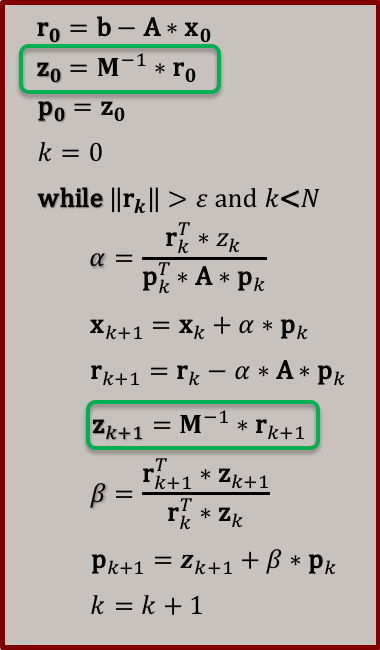
\includegraphics[scale=0.50]{figures/SPARSE-PrecondCGAlg}
      \vspace{-2em}
      \end{center}
  \end{columns}
\end{frame}

\begin{frame}[fragile]{Exercise}
\textbf{Preconditioned CG: Exercise}
\begin{itemize}
  \item Objective:
  \begin{itemize}
    \item Introduce spiluk and sptrsv as preconditioning to a CG solver
    %\item Uses a simple Laplacian matrix on a cartesian grid as a KokkosSparse::CrsMatrix
  \end{itemize}

  \item Exercise and logistics:
  \begin{itemize}
    \item \verb!Exercises/kokkoskernels/CGSolve_SpILUKprecond!
    \item For convenience, use the provided script to install KokkosKernels and generate a Makefile for the code
    \begin{code}
      run_installlibs_cmake.sh
    \end{code}
    \item Change path and build variables as needed based on your setup:
    \begin{itemize}
      \item KOKKOS\_PATH: Point to your Kokkos source directory
      \item KOKKOSKERNELS\_PATH: KokkosKernels source directory
      \item KOKKOS\_DEVICES: Enabled execution spaces
    \end{itemize}
  \end{itemize}

\end{itemize}
\end{frame}

\begin{frame}[fragile]{Exercise}
\textbf{Preconditioned CG: Exercise}
\begin{itemize}

  \item Instructions:
  \begin{itemize}
    \item Search for lines marked "EXERCISE" to apply code changes
    \item Lines marked "EXERCISE hint" give suggestions
    \item Opaque handles already created, SPILUK handle initialized
  \end{itemize}
  \item Key steps:
  \begin{itemize}
    \item Initialize two SPTRSV handles (L and U)
    \item Call spiluk\_symbolic(...) for ILU(k)
    \item Call spiluk\_numeric(...) for ILU(k) factorization
    \item Call sptrsv\_symbolic(...) to do level scheduling for L and U
    \item Call sptrsv\_solve(...) to apply preconditioner during the CGSolve
  \end{itemize}
  \item Observe the convergence behaviors:
  \begin{itemize}
    \item  without preconditioner 
    \item  with preconditioner (as ILU(k) fill-level changes)
    \item  "./cgsolve --help" will show command-line options
  \end{itemize}

\end{itemize}
\end{frame}


\begin{frame}[fragile]{Summary}
\textbf{Summary: SPILUK and SPTRSV}
\begin{itemize}
  \item SPILUK
  \begin{itemize}
    \item Two phase routine, using level scheduling to expose parallelism for the factorization
  \end{itemize}
  \item SPTRSV
  \begin{itemize}
    \item Two phase routine, using level scheduling to expose parallelism for the solve phase
    \item CuSPARSE TPL support is available for NVIDIA GPUs
  \end{itemize}
\end{itemize}

\end{frame}

%==========================================================================

